\section{\"Ubertragung der Messung in die Kavit\"at}
\label{sec:kavitaetueber}
\begin{figure}[htb]
	\centering
	\subfloat[Au\ss{}enansicht der Kavit\"at mit Messaufbau]{\includegraphics[width=0.4\textwidth]{Messung_Kavitaet_NA_crop}}
	\hspace{0.1\textwidth}
	\subfloat[Innenansicht am Gap der Kavit\"at]{\includegraphics[width=0.4\textwidth]{Messung_Gap_Kavitaet}}
	\caption{Messaufbau f\"ur die Messung an der Kavit\"at}
\end{figure}
\begin{figure}[t]
	\centering
	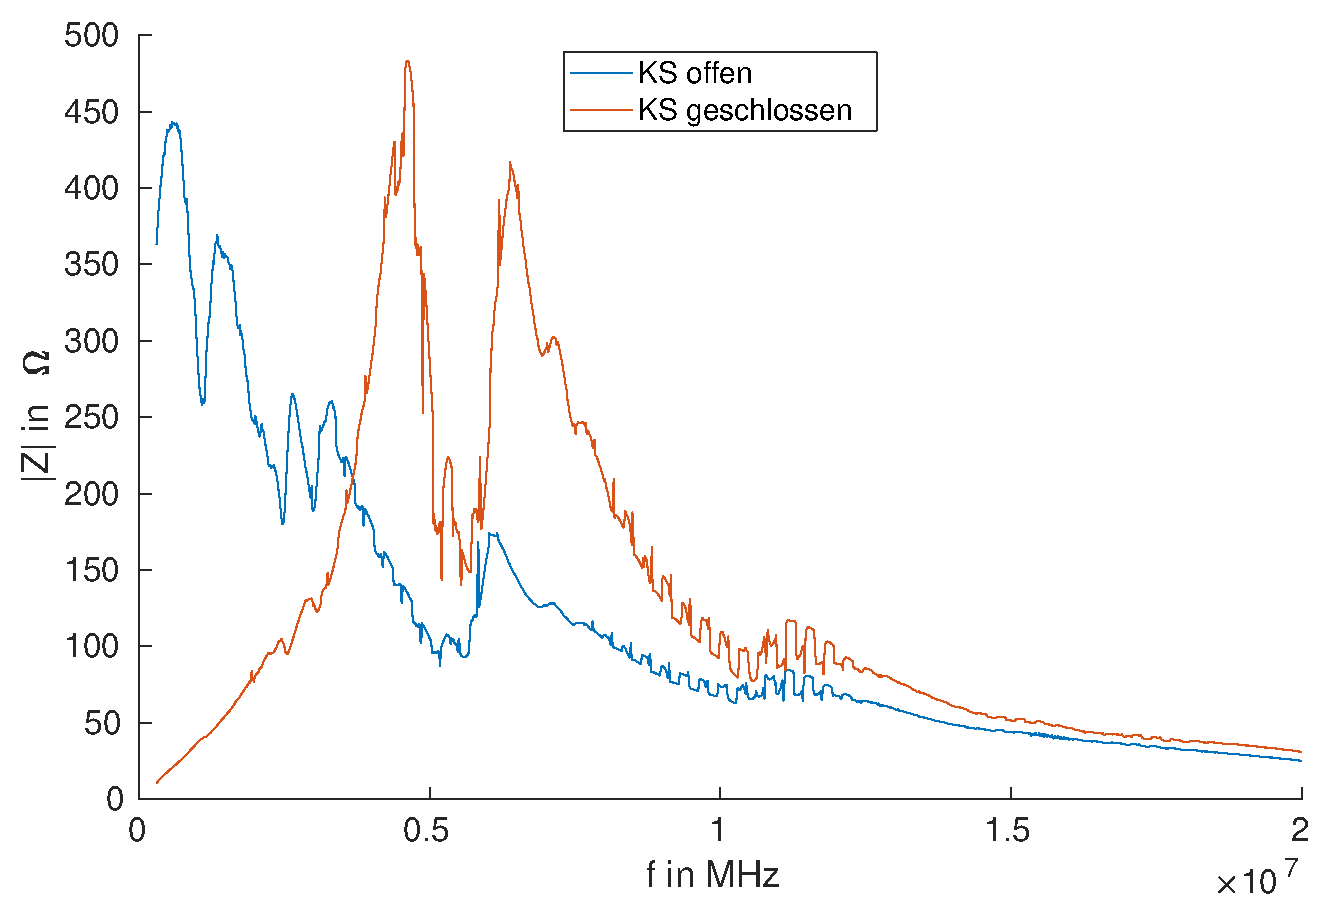
\includegraphics[width=0.6\textwidth]{Z_ges_cavity}
	\caption{Absolutwert der Impedanz gemessen \"uber das Gap in der Kavit\"at Mit geschlossenem Kurzschluss und offenem Kurzschluss.}
\end{figure}